%%「論文」,「レター」,「レター(C分冊)」,「技術研究報告」などのテンプレート
%% 1. 「論文」
%% v3.0 [2015/11/14]

%% 4. 「技術研究報告」
\documentclass[technicalreport]{ieicej}
%\usepackage[dvips]{graphicx}
%\usepackage[dvipdfmx]{graphicx,xcolor}
\usepackage[T1]{fontenc}
\usepackage{lmodern}
\usepackage{textcomp}
\usepackage{latexsym}
\usepackage[dvipdfmx]{graphicx}
\usepackage{graphicx}
\usepackage{amsmath}
\usepackage{txfonts}
\usepackage{url}
\usepackage{enumerate}
%\usepackage[fleqn]{amsmath}
%\usepackage{amssymb}

\setcounter{page}{1}

\jtitle{複数人で使用可能な3Dアイデアノートシステムの提案と実装}
\jsubtitle{}
\etitle{Proposal and Implementation of The 3D Idea Note System for Multiple People}
\esubtitle{}
\authorlist{%
 \authorentry{猪膝 孝之}{Takayuki INOHIZA}{uec}\MembershipNumber{uec}
 \authorentry{田野 俊一}{Shun'ichi TANO}{uec}\MembershipNumber{uec}
 \authorentry{橋山 智訓}{Tomonori HASHIYAMA}{uec}\MembershipNumber{uec}
 \authorentry{丸谷 大樹}{Taiki MARUYA}{uec}\MembershipNumber{uec}
 \authorentry{市野 順子}{Junko ICHINO}{tcu}\MembershipNumber{tcu}
 \authorentry{森 真吾}{Shingo MORI}{tis}\MembershipNumber{tis}
 \authorentry{井出 将弘}{Masahiro IDE}{tis}\MembershipNumber{tis}
% \authorentry[メールアドレス]{和文著者名}{英文著者名}{所属ラベル}
}
\affiliate[uec]{電気通信大学大学院 情報理工学研究科}{Graduate School of Informatics and Engineering, The University of Electro-Communications}
\affiliate[tcu]{東京都市大学 メディア情報学部}{Faculty of Informatics, Tokyo City University}
\affiliate[tis]{TIS株式会社}{TIS Inc.}
\MailAddress{$\dagger$inohiza@uec.ac.jp, $\dagger$tano@is.uec.ac.jp, $\dagger$hashiyama@is.uec.ac.jp, $\dagger$maruya@media.is.uec.ac.jp, $\dagger$$\dagger$ichino@tcu.ac.jp, $\dagger$$\dagger$$\dagger$mori.shingo@tis.co.jp, $\dagger$$\dagger$$\dagger$ide.masahiro@tis.co.jp}
%\affiliate[所属ラベル]{和文勤務先\\ 連絡先住所}{英文勤務先\\ 英文連絡先住所}

\begin{document}
\begin{jabstract}
%和文あらまし
近年、HMD(Head Mounted Display) が普及してきた。現在、HMDに関する研究は一人で使用することを想定していたり、特定の場所で使用することを想定していたり、手やペンで描くのみで入力手法が限定されているものが多い。これらの問題点を踏まえた上で本研究では、複数人で使用可能で、どこでも場所を選ばず利用が可能で、直感的で様々な入力が可能なHMDを使用したシステムの提案を行う。これらのコンセプトに基づいたシステムを設計し、実際にプロトタイプシステムの実装を行った。また、評価実験ではシナリオ実験と課題解決実験の二つを行い、シナリオ実験での手順の遂行状況においてはほとんどの手順において成功率100\%を収めた。課題解決実験においても多くの被験者がタスクを実行できることが確認できた。
\end{jabstract}
\begin{jkeyword}
%和文キーワード
3D, メモ, 共有, マルチモーダル
\end{jkeyword}
%\begin{eabstract}
%英文アブストラクト
%\end{eabstract}
%\begin{ekeyword}
%英文キーワード
%\end{ekeyword}
\maketitle

\section{はじめに}
アイデアはふとしたときに思い浮かぶことがあり、私達はそれを紙に書き留めたり、PCやスマートフォン等を利用してメモを取ることがある。しかし、アイデアが思い浮かぶのは座って作業しているときだけでなく、外で歩いているときや、机やホワイトボード等がないような場面でも突然思い浮かぶことがある。紙とペンを持ち歩いて思い浮かんだらすぐにメモを取る習慣ができてる人はいいが、そうでない人はアイデアが思い浮かんでも「後でメモをすればいいや」と思ってすぐにメモを取ることを諦めてしまうだろう。実際に日頃からアイデアをメモに記録している人は少なくなってきている傾向がある\cite{memo}。思い浮かんだアイデアはできるだけ早くメモを取ったほうが良い。また、アイデアは一人で考えて生み出すものとは限らない。友人との話し合いをしているうちに一人では思いつかなかったアイデアが生まれたり、話が弾んで連鎖的にアイデアが生まれることもある。アイデアを効率的に生み出すための発想法がすでに何種類もあるが、これらの中には複数人で集まって話し合ってアイデアを出すものも多い\cite{hassouhou}。

近年、HMD(Head Mounted Display)が普及してきた。HMDに関する研究はすでに多く行われている。医療技術に関する研究や、デザイナー向けの3Dスケッチに関する研究、他には3D空間上に文字や図形を描いたりする研究等もある。近年ではMRも流行化してきており、医療診断・手術計画や屋内外の誘導・案内、埋蔵物確認、都市計画・建築分野でのシミュレーション、アミューズメント産業等の応用分野から大きな期待がされている\cite{mr}。

現在、HMDに関する多くの研究は一人で使うことが想定されている。また、特定の場所において使用することを想定している場合も多い。そして、手やペンで描くのみで入力手法が限定されている場合も多い。現状では複数人で使用することを想定していたり、外などの広い空間で利用することを想定していたり、手で描くだけでなく音声でも入力可能なシステムを想定している研究やアプリケーションは少ない。そこで、複数人で使用できて、どこでも利用できて、様々な入力ができるシステムが必要だと考え、本研究の立案に至った。

\section{従来研究と問題点}
椎尾ら\cite{siio}, \cite{siio2}は仮想の手書きメモによるコミュニケーションをウェアラブルコンピュータにより実現する空気ペンを試作した。問題点としては、同時に複数人で使用できないことや、使用できる範囲がRFIDタグがついた床上のみなので場所が限定されることが挙げられる。

また、高山ら\cite{tano}, \cite{tano2}は実世界のどのような時間・場所であっても、ユーザが思い浮かんだふとしたアイデアを、生起を誘発したコンテキストに対応づけて保存し、それを他のユーザと共有できるシステムを作成した。問題点としては、多くの機器を装着しなければならないので持ち運びが大変であることや、操作が複雑なので慣れるのに時間がかかることが挙げられる。

長田ら\cite{nagata}はスマートグラスを用いた仮想空間への手書き情報共有システムを提案した。問題点としては、指のみの操作だとできることが限定されることが挙げられる。

従来研究のHMDを使用したシステムの問題点をまとめると以下である。

\begin{itemize}
 \item 同時に複数人で使用することを想定していない
 \item 利用できる場所が限定されている
 \item 入力手法が限定されている
\end{itemize}

\section{本研究のコンセプト}
本章では、前章で述べた問題点を踏まえた上でシステムコンセプトを述べる。

\subsection{システムコンセプト}
従来研究のHMDを使用したシステムでは同時に複数人で使用することを想定していない、利用できる場所が限定されている、入力手法が限定されているという問題点があった。

そこで、従来研究の問題点を踏まえ、本研究は以下の三つを満たすようなHMDを使用したシステムを提案する(図\ref{fig:concept})。

\begin{enumerate}
 \item 複数人で同時に使用することが可能
 \item どこでも場所を選ばず利用が可能
 \item 簡単な操作で直感的で様々な入力が可能
\end{enumerate}

\begin{figure}[h]
  \begin{center}
    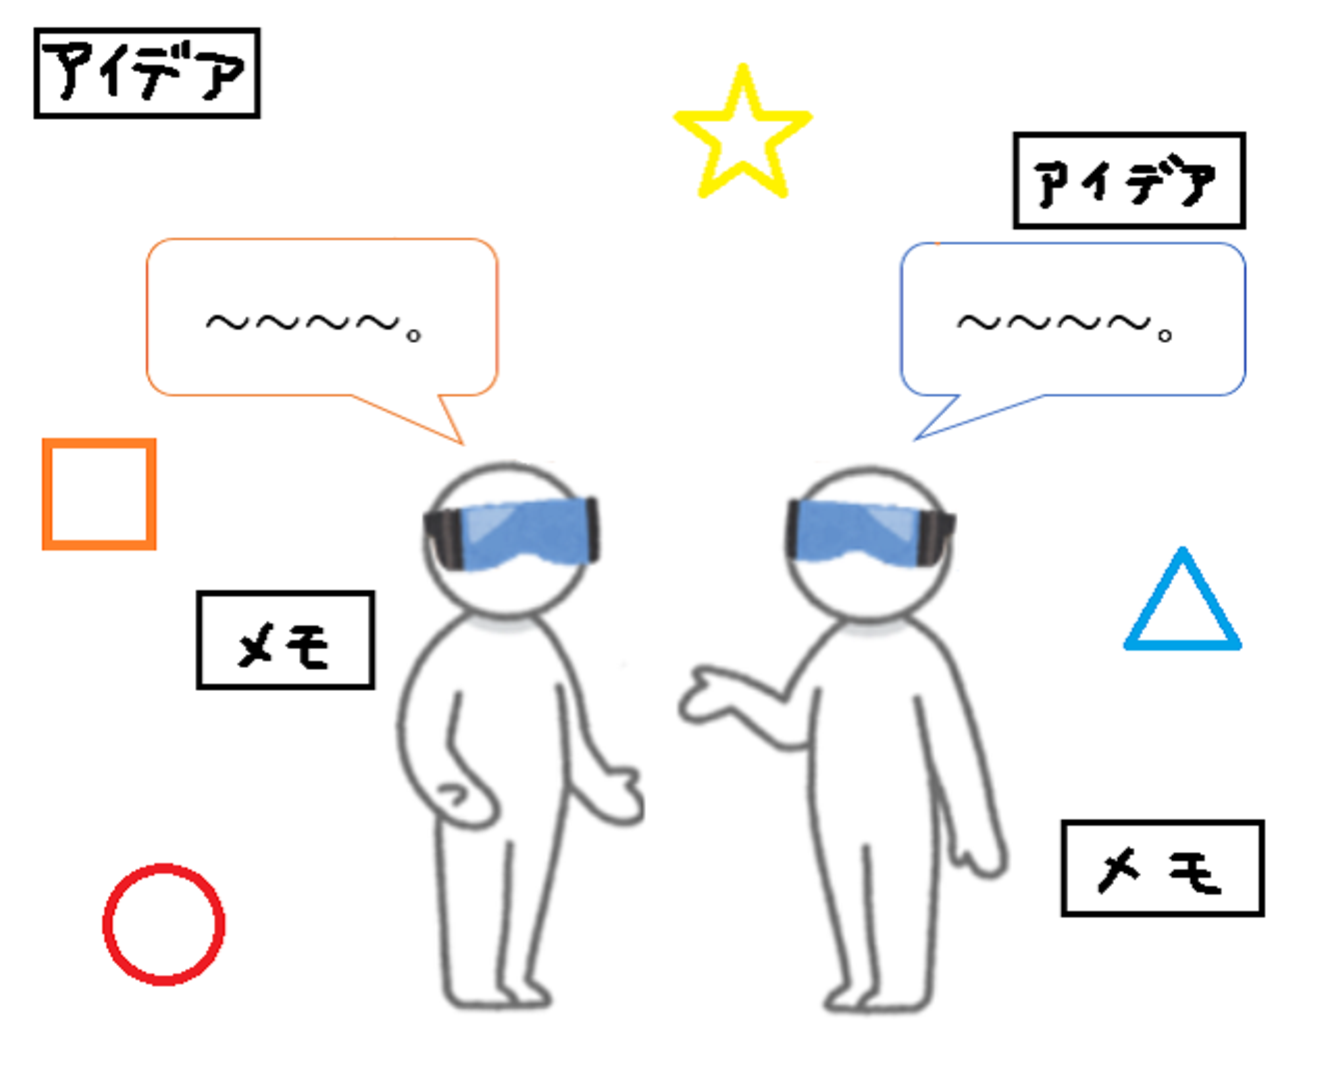
\includegraphics[clip,height=6.0cm,width=7.0cm]{./concept.eps}
    \caption{システムコンセプト}
    \label{fig:concept}
  \end{center}
\end{figure}

\subsection*{特徴1:複数人で同時に使用することが可能}
既存の研究では一人で使用することを想定したシステムが多かった。または、将来的には複数人で使用できるようにすることを目標にしてるが現状のシステムでは一人でしか使用できないというものも多かった。他には、複数人で使用することはできるが同時に使用することができないというものあった。アイデアは一人で考えて生み出す場合もあるが、複数人で集まって話し合って一緒に考えることによってアイデアが生まれることもある。ある人がアイデアを出せば、そのアイデアに対して他の人が反応して新たな意見を出して、そこからまた新しいアイデアが生まれることもある。それが連鎖的に続くことによって結果的にアイデアをたくさん生み出すことに繋がる。アイデアを効率的に生み出す方法が既に何種類も存在するが、その中には実際に複数人で集まって話し合ってアイデアを出し合うというものも多い。したがって、複数人で同時に使用できて、お互いのメモをリアルタイムで共有できることが必要不可欠である。また、複数人で利用する際に空間上に文字を残す場合に問題点が発生する。その問題点については\ref{moji_mondai}節で詳しく述べる。

\subsection*{特徴2:どこでも場所を選ばず利用が可能}
既存の研究では机やPCの近く、または特定の場所等のみでしか使用できないシステムが多かった。他には、どこでも利用可能ではあるが多くの機器を装着しなければならなかったり等、可搬性に問題があるシステムもあった。アイデアが生まれるのは椅子に座って机で作業しているときや、黒板やホワイトボードの前に立っているとき等、何かノート等を使ってメモを取ることができる場所だけとは限らない。アイデアは思いがけない場所でふとしたときに突然思い浮かぶことがある。時には外で歩いているときや、軽い運動をしているときに思い浮かぶこともある。実際に動きながらメモを取るのは困難である。また、普段から常にメモ帳等を持っていてすぐにメモを取る習慣がついている人は良いが、そうでない人はメモを取ることを諦めてしまったり、後回しにしまいがちである。アイデアが思い浮かんだら、当然すぐにメモを取るほうが良い。したがって、どこでも場所を選ばずに利用できるようなシステムが必要である。

\subsection*{特徴3:簡単な操作で直感的で様々な入力が可能}
既存の研究では空間上で描くのみ等で入力手法が限定されているシステムが多かった。または、特別なジェスチャを定義して使用する必要があったり、慣れるのにかなり時間がかかる等のシステムもあった。アイデアの形は文字や図形等、様々な形をとる。立体的な形を持ったアイデアもあれば、平面の形を持ったアイデアも存在する。仮に入力手法を空間上に描くのみにした場合、考えたアイデアが短い文章にまとまらないときメモを取ることが困難である。また、仮に入力手法を音声のみにした場合、シンプルな図形であれば表示できるかもしれないが、大きさを音声入力で指定しなければならなかったり、複雑な図形を描く際は困難である。したがって、簡単な操作で直感的で様々な入力ができるシステムが必要である。

\subsection{文字を表示する上での問題点と解決案} \label{moji_mondai}
複数人で空間上に文字のメモを残す際に、見る視点によって文字として見えないという問題点が発生する。解決案として、文字を動的に相手の方向に回転させて向けたり、文字のメモに触れたら自分の前に見えるように表示する等の方法が考えられる。しかし、文字を動的に相手の方向に回転させて向けてはいけない場合もある。それは、平面上に文字のメモを残した場合である。何故ならばその平面そのものに意味があるからである。このようなメモの表示に関しての解決案は、その平面上に残した文字のメモに目線を合わせて、それ自体はそのままにしておき、その平面上に残した文字を目の前等の自分の見やすい位置に表示するという手法を提案する。

また、平面の形を持った文字以外に立体的な形を持つ文字が存在すると考えられる。立体的な文字に関してはそれ自体に意味を持つので回転したり等はしないほうがよいと考えられる。

\section{システム設計}
本研究のコンセプトで述べたシステムコンセプト(1)、(2)、(3)を踏まえた上でシステムの全体構成について述べる。その次にそれぞれの機能の設計に関して詳しく説明する。また、ハードウェアは可搬性を考慮して、マイクロソフト社のHoloLens\cite{hololens}を使用する。

\subsection{全体構成}
(1)複数人で同時に話し合って使用できてお互いのメモを共有できるようにするために、サーバを介して空間を共有する機能が必要である。(2)どこでも場所を選ばずに利用できて、実世界の広い空間上に任意の場所にメモを置く際には、遠くにあるメモに対して操作する機能が必要である。また、(3)簡単な操作で直感的で様々な入力を可能にするには、3D空間上に描画する機能だけではなく、音声でも入力ができることが必要である。以上より、システムの機能としては大きく分けて、メモを入力、メモを操作、メモを共有の三つであり、以下に詳細を述べる。

\subsection{メモを入力}
実世界の任意の3D空間上に図形や文字のメモを描いて残したり話して残したりできるようにする。3D空間上に文字によるメモを相手に見えるようにするためには回転して相手に向けるという手法が考えられる。しかし、平面に残したメモの場合、その面自体に意味があるので回転させてはならない。そこで、正面からメモを見た場合はそのまま表示し、ある程度横から見た場合にはそのメモ自体はそのままだが、内容がわかるように目の前に見やすく表示をするという手法を提案する。(図\ref{fig:memo_wall})

\begin{figure}[h]
  \begin{center}
    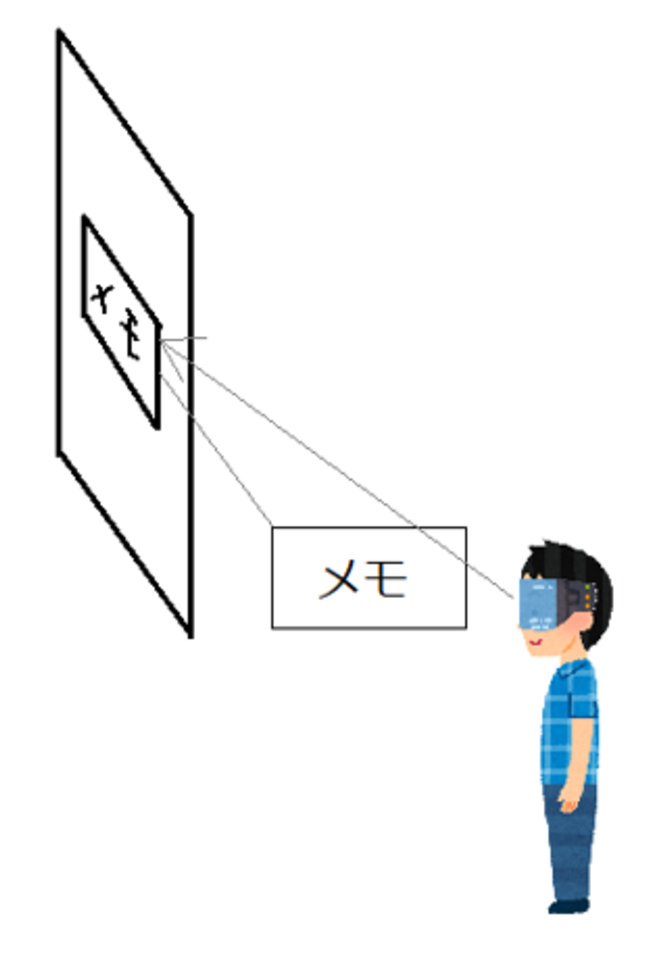
\includegraphics[clip,height=6.0cm,width=4.0cm]{./memo_wall.eps}
    \caption{ある程度横から見た場合は目の前にも表示}
    \label{fig:memo_wall}
  \end{center}
\end{figure}

\subsection{メモを操作}
広い空間上にメモを残す場合、遠くに配置してあるメモをどうやって選択、移動、削除するかという問題が発生する。そこで、以下の三つのインタラクションを提案する。

\begin{enumerate}[(1)]
 \item ルームスケールチェンジ
 \item 3Dラバーバンド
 \item 3Dフィッシング
\end{enumerate}

(1)手元に部屋全体を縮小したものを用意してメモを操作する手法で、(2)はイメージとしては手元に輪ゴムがついたオブジェクトを引っ張って遠隔のメモを操作する手法、(3)は視線と手元のオブジェクトを利用して釣りのように遠隔のメモを操作する手法である。

\subsection{メモを共有}
実世界の任意の3D空間上に残したメモを対面にいる人だけでなく、遠隔にいる人にもメモを共有できるようにする。遠隔にいる人はアバターを実世界に表示させる。

\section{プロトタイプシステムの実装}
設計したシステムを基に行ったプロトタイプシステムの実装について述べる。

\subsection{プロトタイプシステムの構成}
設計されたシステムは、ユーザがシステムの各機能を利用するために使うアプリケーションと、HoloLens同士で相互接続するためのサーバ、ユーザが喋った内容をテキストに変換するクラウドサービスが存在する。図\ref{fig:prototypesystem1}にプロトタイプシステムの全体図を示す。以下でそれぞれについて述べる。

\begin{figure}[h]
  \begin{center}
    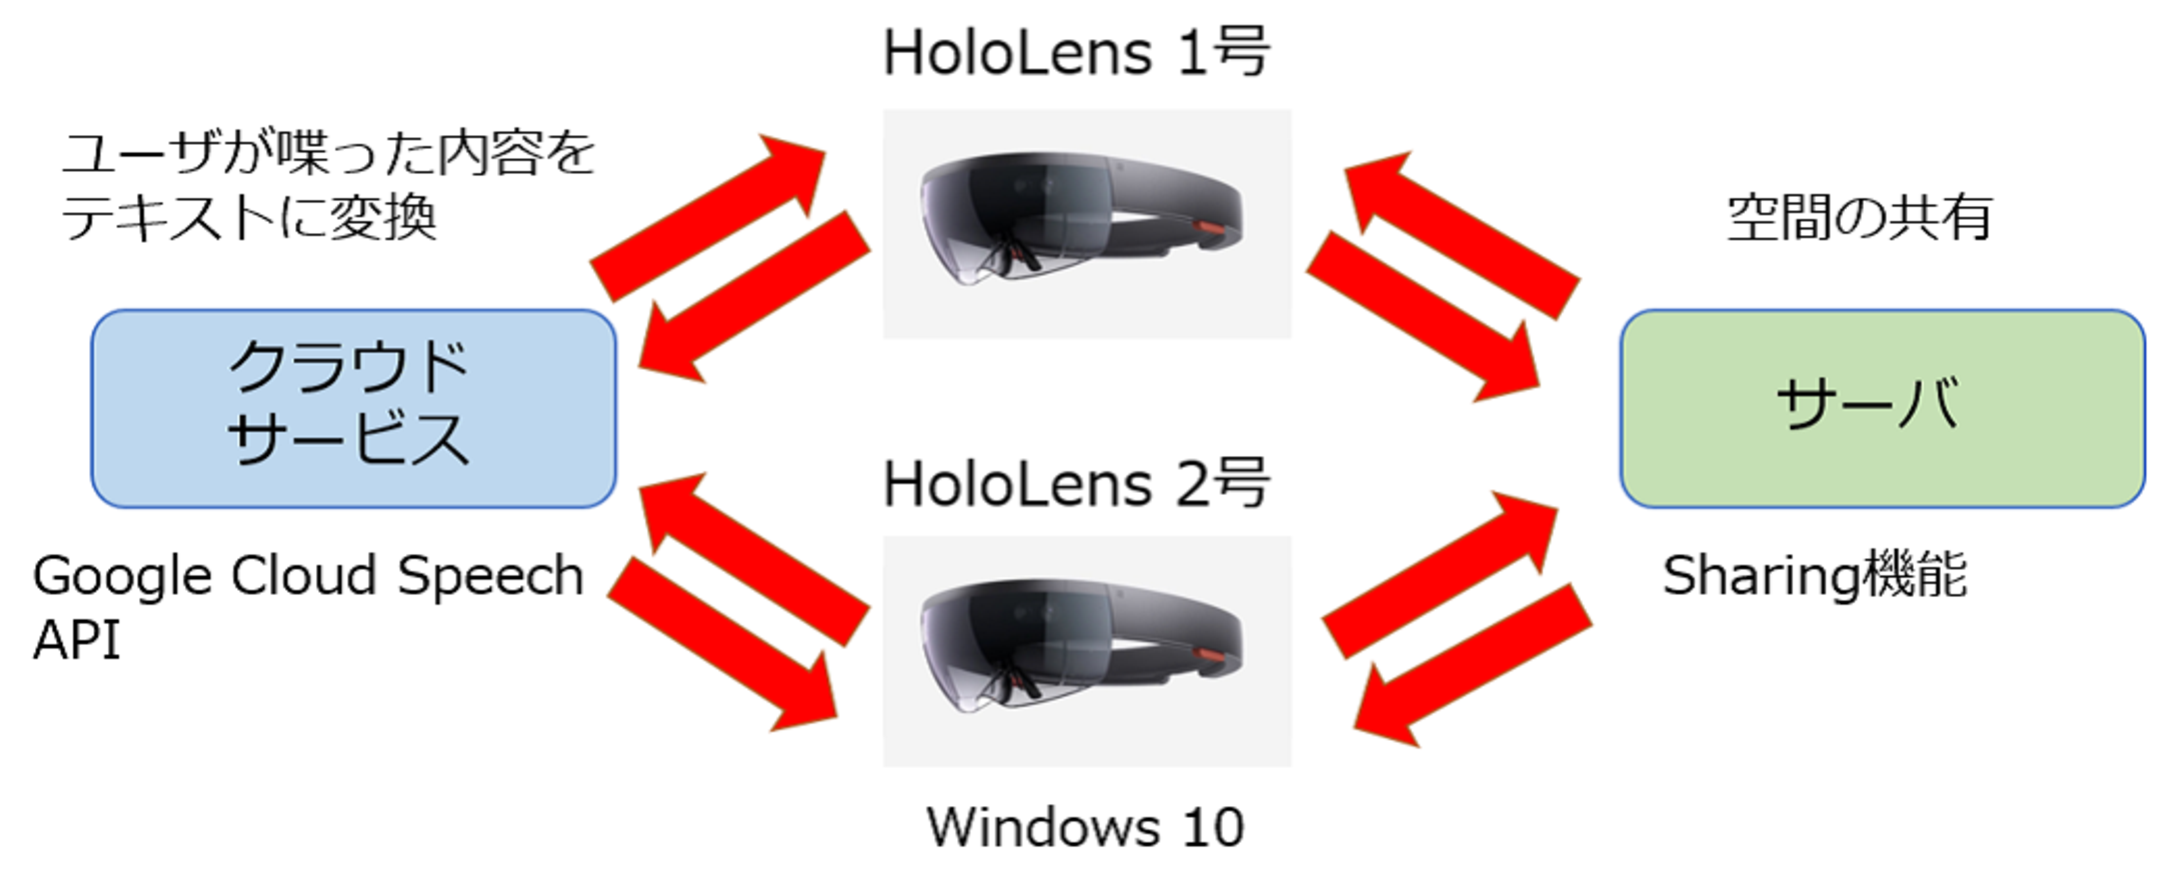
\includegraphics[clip,height=4.0cm,width=9.0cm]{./prototypesystem1.eps}
    \caption{プロトタイプシステムの構成}
    \label{fig:prototypesystem1}
  \end{center}
\end{figure}

\subsubsection{アプリケーション}
Windows 10やWindows 10 Mobile上で動作するUWP(Universal Windows Platform)アプリとして作成すると、HoloLens上でもそのアプリケーションが動作する。アプリケーションの開発には、マイクロソフト社が配布している統合開発環境であるVisual Studio 2017(Ver 15.0)と、ユニティ・テクノロジーズ社が配布している統合開発環境を内蔵した複数のプラットホームに対応するゲームエンジンであるUnity(Ver 5.6.2f1)を使用した。また、Unity 用のHoloLens 向けのツールキットであるHoloToolkit-Unity\cite{holotoolkit}の導入を行った。開発言語には、Windows向けのアプリケーションの開発に主に使われるC\#を採用した。

\subsubsection{サーバ}
実世界の任意の空間上に残したメモを他のHoloLensを使用している人と共有するには、HoloToolkitのSharingという機能を利用し、Sharing用のサーバを介して空間の共有を行った。HoloLensの座標系は特殊であり、このまま共有をしても現実の空間の同じ位置で物体を共有することはできないという問題が発生する。この問題を解決するためにはアンカーの共有を行った。アンカーとは船の錨の意味で空間内の絶対的な位置に居座ることができるオブジェクトのことである。これを設置することで位置合わせを行い、実世界の任意の空間上に残したメモの共有を行った。

\subsubsection{クラウドサービス}
HoloLensの標準機能で音声入力はサポートされているが、現在利用できる言語が英語のみである。そこでGoogle Cloud Speech API\cite{google_speech}を利用することにより、日本語の音声をテキストに変換する。Google Cloud Speech APIとはGoogleの持つ音声認識技術を使用し、音声をテキストに変換するサービスである。

\subsection{プロトタイプの実装}
プロトタイプシステムの機能は全てで四つである。機能を選択後は音声入力またはキーボードを使用してメニュー画面に戻ることができる。3D描画モードでは3D空間上で目の前でタップ&ホールドをすると描画が開始され、ホールドを解除すると描画をやめる。付箋モードでは喋った内容をテキスト化して付箋として目の前に残す。また、壁に貼り付けることも可能である。Voice Lineモードではタップ&ホールドをして線を引きながら喋って、引いた線上にテキスト化してメモとして残す。首振りモードでは首を縦または横に振ると頭上に文字の表示を行う。

%\begin{figure}[h]
%  \begin{center}
%    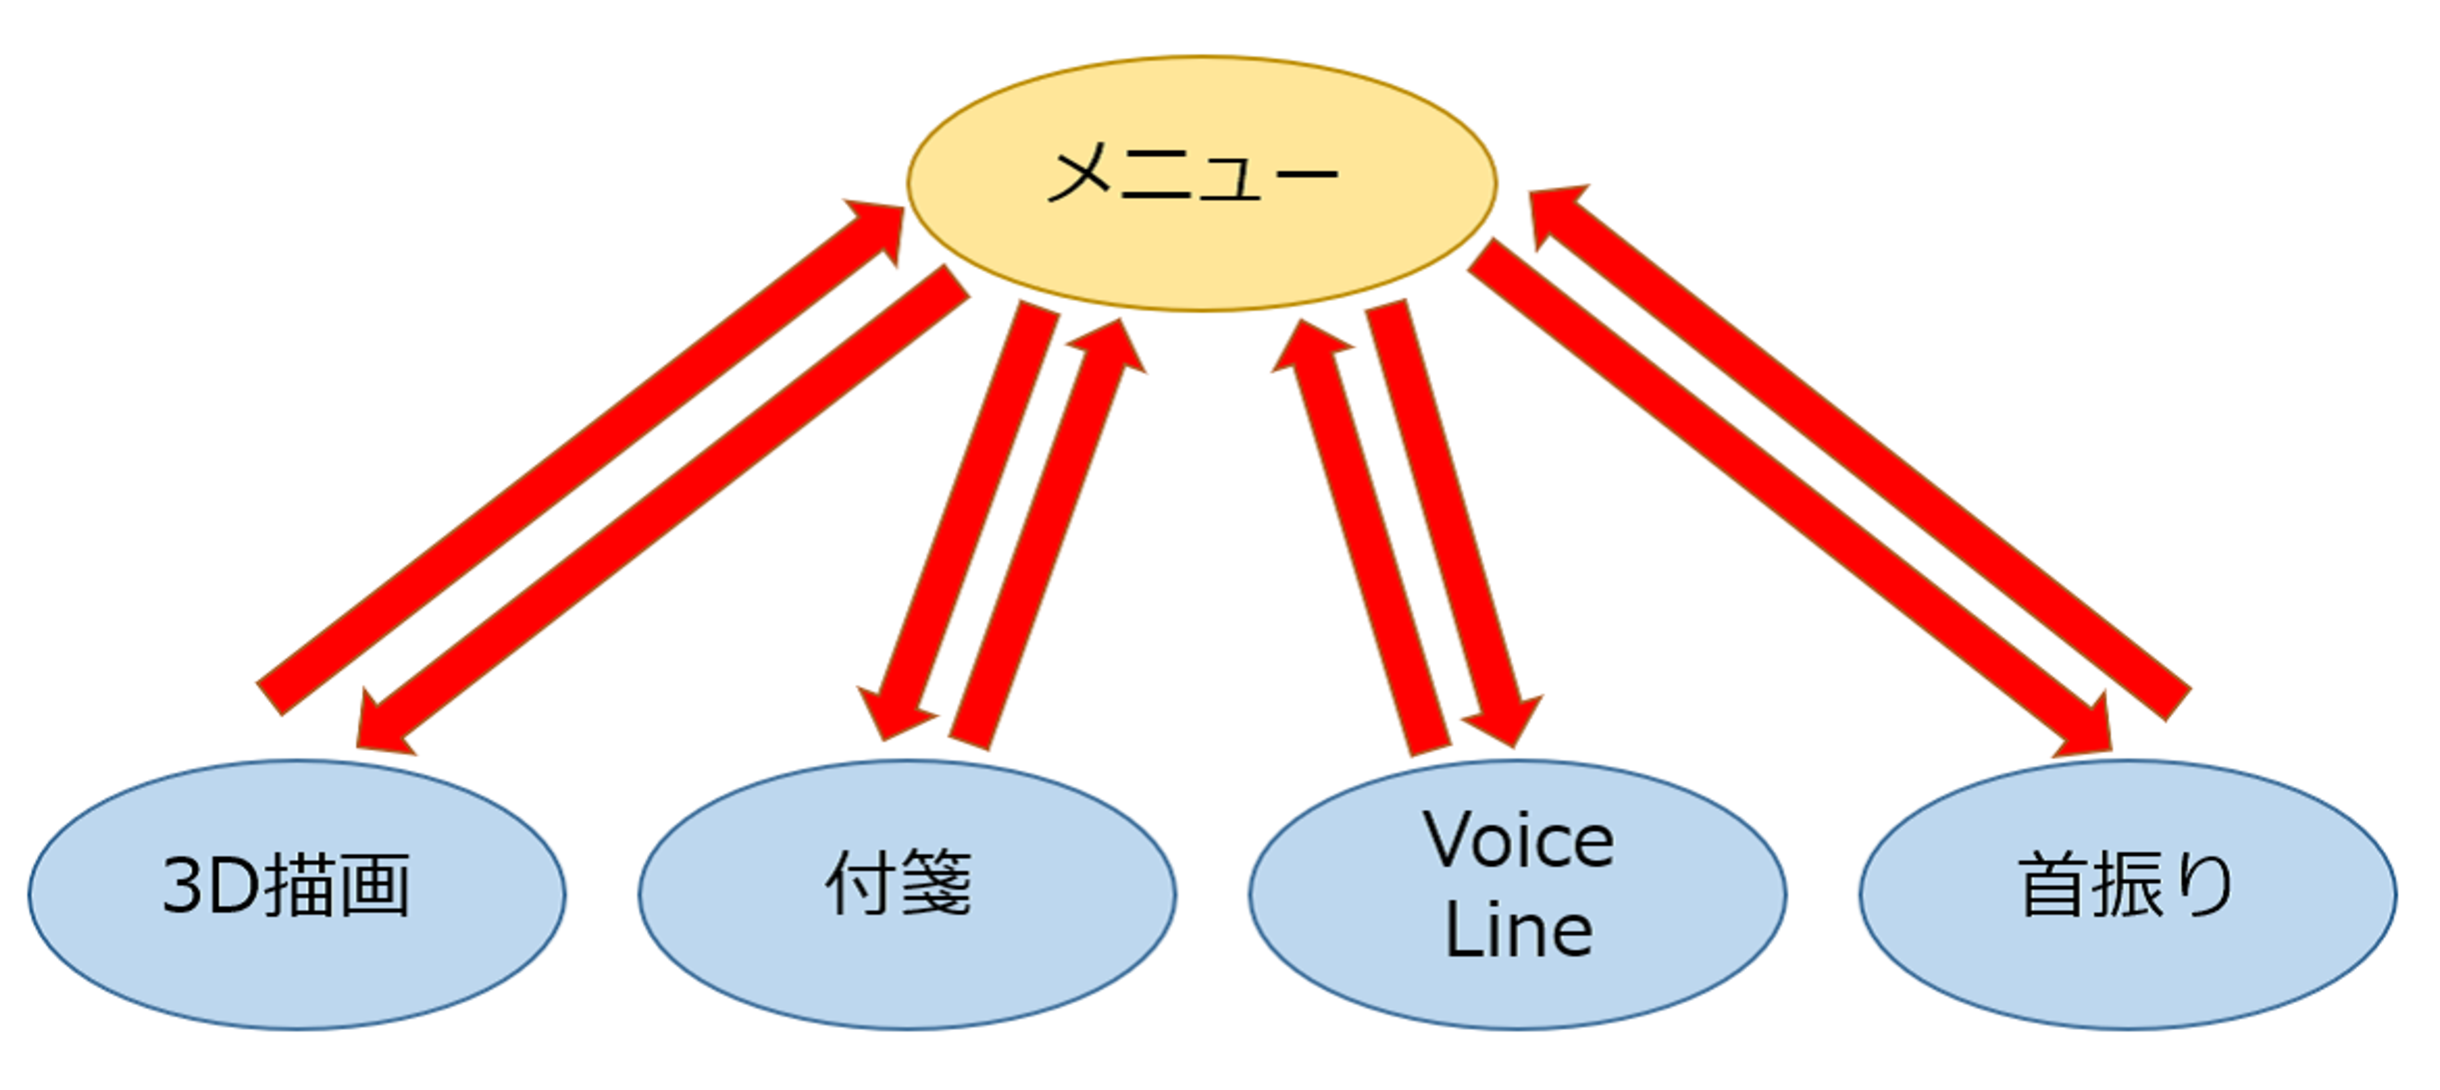
\includegraphics[clip,height=4.0cm,width=8.0cm]{./senizu.eps}
%    \caption{システムの遷移図}
%    \label{fig:senizu}
%  \end{center}
%\end{figure}

\section{プロトタイプの評価実験}
本章では、実装したプロトタイプシステムの評価のために行った実験について述べる。

\subsection{実験の目的}
本実験は実装したプロトタイプシステムの機能が正常に動作するかどうかの確認を行うことと、システムに実装されているそれぞれの機能をユーザに使用してもらうことで提案システムの有用性について検証を行うことの2つを目的としている。

\subsection{実験の被験者}
本実験の被験者は男性9人と女性1人の合計10人で、情報系を専攻する大学生および大学院生である。平均年齢は23.7歳で、右利きの人が7人で左利きの人が3人である。HoloLensの使用経験について、全くないと回答したのが4人、少しあると回答したのが5人、よく使うと回答したのが1人である。

\subsection{実験環境}
本実験では実装したプロトタイプシステムのアプリケーションを2台のHoloLensにそれぞれインストールして用意をした。また、共有を行うためなるべく確実にネットワークに接続ができるように研究室内のゼミ室で行った。この実験では、被験者2人で1グループとして同時に行った。実験中に取り組んでもらうタスクに関する説明は、それぞれの被験者に渡せるように資料を作成して用意した。また、システムの機能の一部でキーボードを使用する箇所があるため、2つのBluetoothキーボードを用意した。

実験中の様子を図\ref{fig:jikkenchu}に示す。

\begin{figure}[h]
  \begin{center}
    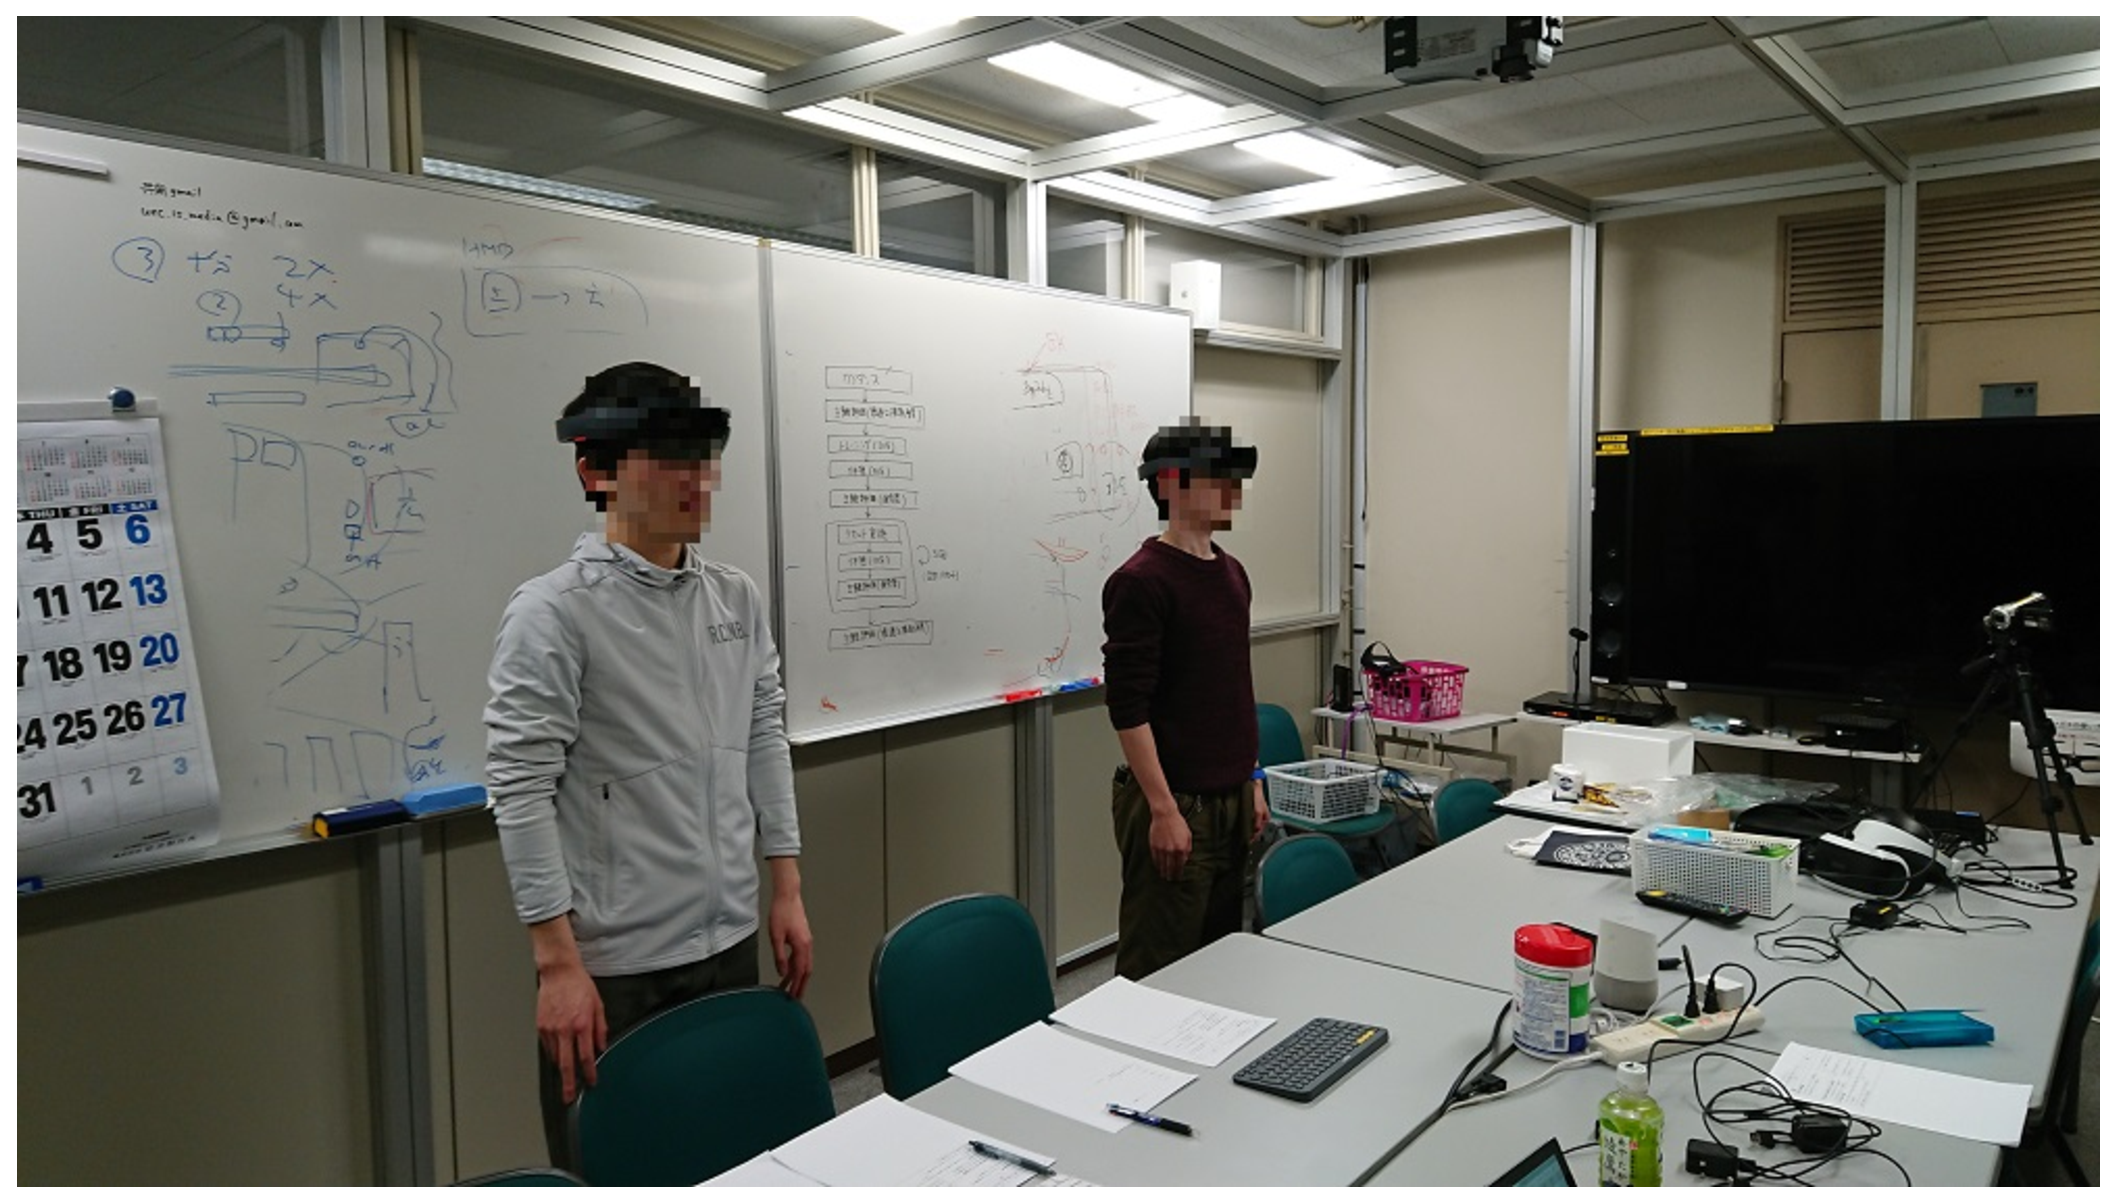
\includegraphics[clip,height=4.0cm,width=7.0cm]{./jikkenchu.eps}
    \caption{実験中の様子}
    \label{fig:jikkenchu}
  \end{center}
\end{figure}

\subsection{実験方法}
本実験は以下に示す2つの作業から構成される。

\begin{itemize}
 \item シナリオ実験
 \item 課題解決実験
\end{itemize}

HoloLensを2台使用して共有を行うためそれぞれのタスクの前に準備を行った。それぞれで定められたタスクに取り組んでもらい、システムの動作状況やタスクの遂行状況などを確認して記録を行った。全てのタスクが終了した後に、プロトタイプシステムに関するアンケートに回答してもらった。各実験の詳細な手順についてを以下で述べる。

\subsubsection{準備}
それぞれのタスクを実際に行っていく前に、2台のHoloLensで共有を行うための準備を行った。まず1人目の被験者に所定の座席に座ってもらい、前方にある予め設置した壁の図形を見てもらいながらHoloLensをかぶってアプリケーションを起動してもらった。1人目の起動が完了したら一度その座席から離れてもらい、2人目の被験者にも同様にその座席に座って前方にある図形を見てもらいながらアプリケーションを起動してもらった。2人目の起動が完了したら、それぞれのタスクに取り組んでもらうようにした。

\subsubsection{シナリオ実験}
シナリオ実験では、決められた手順に従ってそれぞれの被験者に操作をしてもらう。この手順は、プロトタイプシステムに実装されている全ての機能を使うように作られている。また、2人で同時に行って共有を行うため、一つの手順が終わったらそれぞれの被験者に完了したことを言うようにしてもらう。表\ref{table:task1}~\ref{table:task4}にシナリオの流れを示す。この4つのタスクを一通り実施することで、プロトタイプシステムに実装されている機能の全てを体感することができる。

\begin{table}[h]
\caption{タスク1:3D描画モードを使用した入力、共有}
\label{table:task1}
\begin{center}
\begin{tabular}{|c|c|}
\hline
手順 & 内容  \\
\hline\hline
1 & 準備  \\
\hline
2 & 空間上に線を描画  \\
\hline
3 & 相手が描いた線が共有できているか確認 \\
\hline
4 & 描いた線を全て削除  \\
\hline
\end{tabular}
\end{center}
\end{table}

\begin{table}[h]
\caption{タスク2:付箋モードを使用した入力、操作、共有}
\label{table:task2}
\begin{center}
\begin{tabular}{|c|c|}
\hline
手順 & 内容  \\
\hline\hline
1 & 準備  \\
\hline
2 & 空間上に付箋のメモを残す  \\
\hline
3 & 付箋の共有 \\
\hline
4 & 付箋の削除  \\
\hline
5 & 付箋のメモを残して共有  \\
\hline
6 & 付箋の移動 \\
\hline
7 & 付箋を壁に貼る \\
\hline
\end{tabular}
\end{center}
\end{table}

\begin{table}[h]
\caption{タスク3:Voice Lineモードを使用した入力、共有}
\label{table:task3}
\begin{center}
\begin{tabular}{|c|c|}
\hline
手順 & 内容  \\
\hline\hline
1 & 準備  \\
\hline
2 & 線が表示されるか確認  \\
\hline
3 & 発声してメモを入力して共有 \\
\hline
4 & メモを全て削除  \\
\hline
\end{tabular}
\end{center}
\end{table}

\begin{table}[h]
\caption{タスク4:首振りモードを使用して頭上の文字を確認}
\label{table:task4}
\begin{center}
\begin{tabular}{|c|c|}
\hline
手順 & 内容  \\
\hline\hline
1 & 準備  \\
\hline
2 & 実験者の指示に従って首振り動作を行う  \\
\hline
\end{tabular}
\end{center}
\end{table}

\subsubsection{課題解決実験}
課題解決実験では、シナリオ実験のような詳細な操作手順は用意しない。代わりに簡単な課題を被験者に出して、プロトタイプシステムを用いてその課題を解決するように指示した。被験者は、先に実施するシナリオ実験においてプロトタイプシステムの操作を一通り終えているので、被験者が自ら考えてプロトタイプシステムを操作して課題を解決することになる。

\subsection{実験結果と考察}
ここではシナリオ実験、課題解決実験の結果と考察について述べる。また、アンケート結果についても記述する。

\subsubsection{シナリオ実験の結果}
タスク1~4のほとんどの手順で成功率が100\%となった。また、支障なくタスクの完了ができないという報告が3件あったが、全てハードウェア上の問題が原因だと考えられる。その3件に関しては、被験者には実験者からの助言を元に手順を行ってもらい、問題なく完了させることが確認できた。

\subsubsection{課題解決実験の結果}
タスク5~7は課題解決実験である。この実験ではシナリオ実験のような詳細な操作手順は用意しない。手元にある資料の文章を読んでもらい、自ら考えて課題を行ってもらった。実験結果としては、全ての被験者が問題なくプロトタイプシステムを使用してタスクを完了できることが確認できた。

\subsubsection{アンケートの結果}
アンケート結果を図\ref{fig:question1}, \ref{fig:question2}に示す。番号1.1~1.6が3D描画モードについての質問、番号2.1~2.9が付箋モードについての質問、番号3.1~3.7がVoice Lineモードについての質問、番号4.1~4.3が首振りモードについての質問、番号5がこのシステム全体についての質問である。質問は5段階評価になっていて、全くそう思わない(1pt)~そう思う(5pt)で平均値を計算している。

3D描画モードについての質問に関しては、番号1.2が平均値2.9と評価が低かった。番号1.2は線が描こうとしたところに正しく表示されているかどうかを問うものである。システムとハードウェアの仕様上、タップする場所の検知はあまり正確ではなく、精度が悪いと感じた被験者が多かったことがわかる。先ほども述べたが、線の描画される位置を少し補正する等の処理が必要だったと考えられる。番号1.3が平均値4.8とかなり高い評価であった。番号1.3は線の共有ができたかどうかを問うものである。結果より共有に関しては問題なかったことがわかる。番号1.4が平均値3.8だが、意見が大きく分かれてた。番号1.4は線の削除を音声入力またはキーボード入力で行えたかどうか問うものである。全ての被験者が音声入力での削除に失敗をしていたため、最初からキーボード入力に限定すべきであった。英語での発音は難しく、またシステムの仕様上音声認識が内部で複数動作していることが失敗率を高くしてしまう原因だと考えられる。

付箋モードについての質問に関しては、番号2.4を除いて平均値4.0以上と全体的に高い評価になった。番号2.4は付箋の削除ができたかどうかを問うものである。理由としては3D描画モードの削除と同様である。番号2.1が平均値4.7とかなり高い評価になった。番号2.1は付箋を残すことが簡単にできたかどうかを問うものである。結果からこの入力方法はほとんどの人が直感的で簡単に入力できることがわかった。番号2.3が平均値4.9と一番高い評価となった。番号2.3は付箋の共有が簡単にできたかどうかを問うものである。これより共有に関しては問題がなかったことがわかる。

\begin{figure}[h]
  \begin{center}
    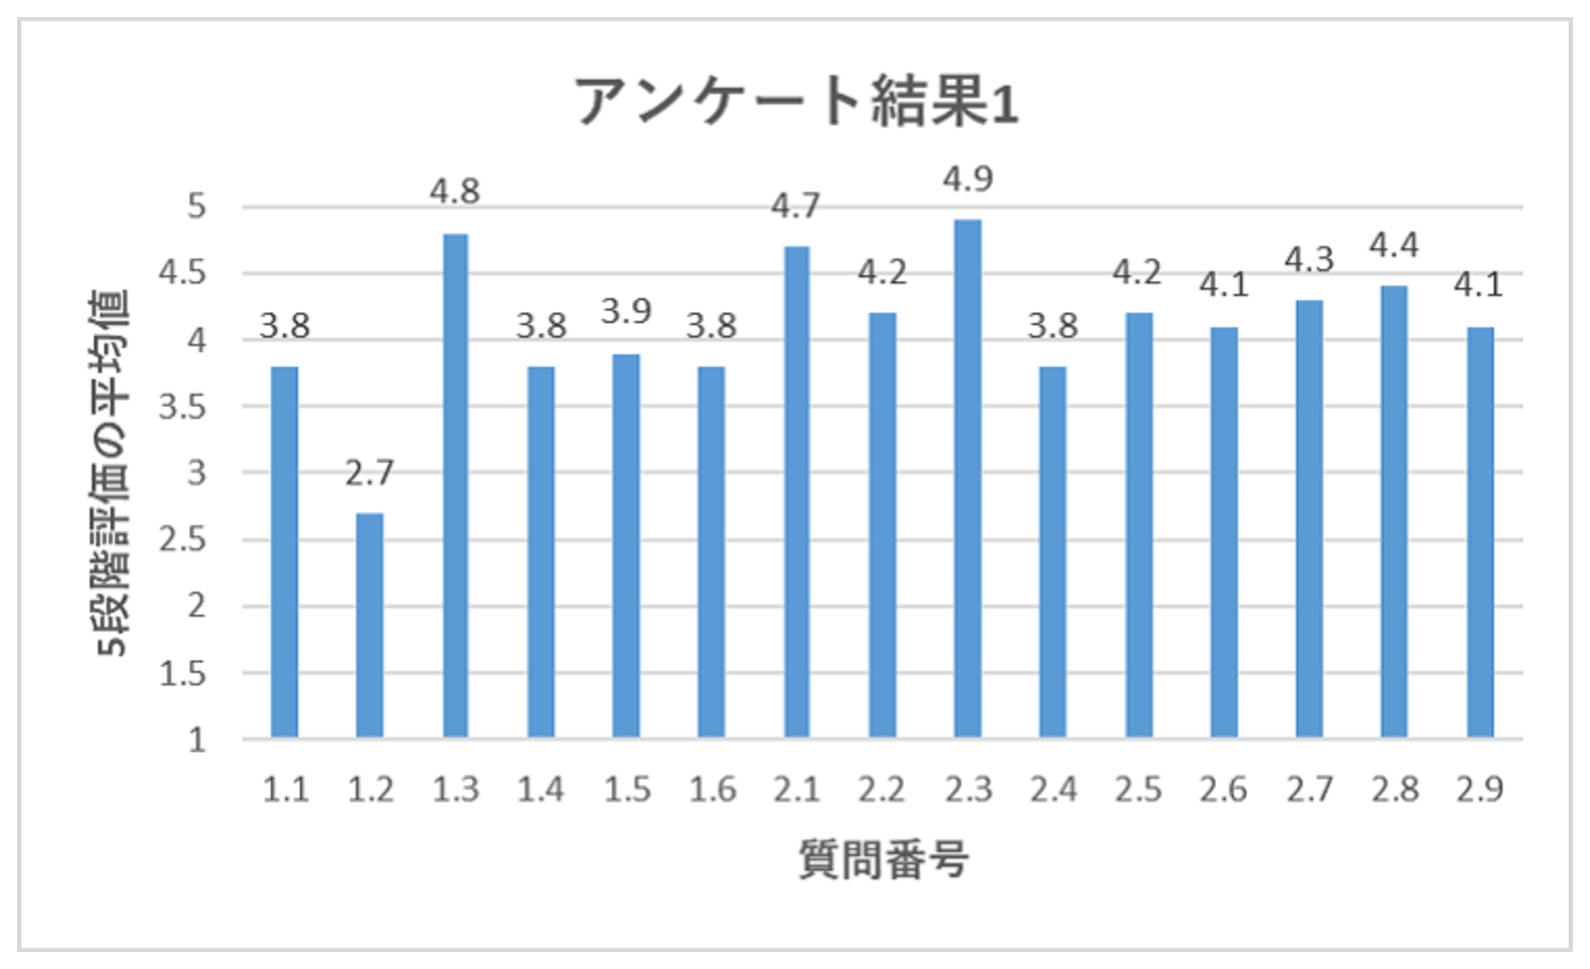
\includegraphics[clip,height=6.0cm,width=9.0cm]{./question1.eps}
    \caption{アンケート結果1}
    \label{fig:question1}
  \end{center}
\end{figure}

Voice Lineモードについての質問に関しては、番号3.3が平均値3.5とやや評価が低かった。番号3.3はメモの位置が正しい場所に表示されていたかどうかを問うものである。理由としては3D描画モードの表示位置のときの場合と同様である。番号3.4が平均値3.8だが、意見が大きく分かれていた。番号3.4はメモの削除ができたかどうかを問うものである。理由としてはこれも3D描画モードの削除の場合と同様である。番号3.7が平均値3.6とやや評価が低かった。番号3.7は普段描きづらいと思うような場所にもメモを残すことができたどうかを問うものである。これ関しては人によって異なるという感じであった。タップの検知する精度が良くなり正しい場所にメモが表示されていたら、もっと評価が高くなったのではないかと考えられる。

首振りモードについての質問に関しては、他の機能と比較すると全体的に評価が低かった。

この機能をまた使用したいかどうかの質問は番号1.6、2.9、3.7、4.3である。結果より付箋モードは多くの被験者にとって使いやすいと感じるということがわかった。また、3D描画モードとVoice Lineモードは人によって異なるという感じであったので、メモの表示位置がもう少し良くなれば評価が変わったのではないかと考えられる。首振りモードに関しては評価が低かった。この機能はまだ完全なものではなく、改善が必要だと改めて感じた。最後に番号5が総合的に見てこのシステムをまた使用したいかどうかを問うものであるが、それなりに評価が高く、このシステムがだいたいの人から受け入れられていることがわかった。

\begin{figure}[h]
  \begin{center}
    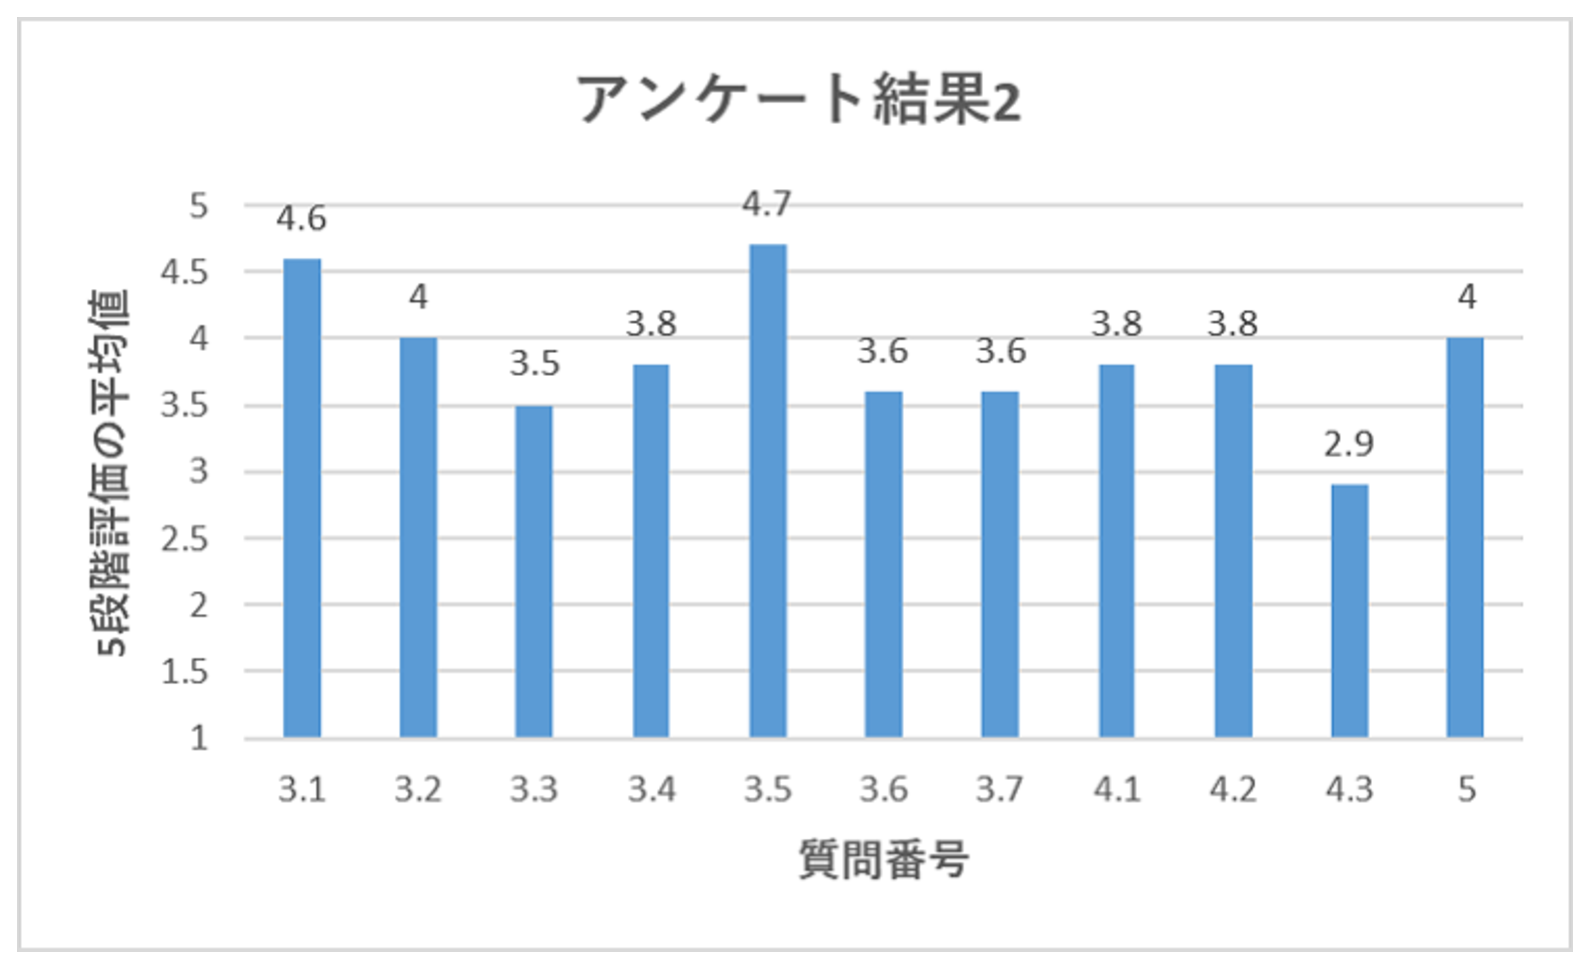
\includegraphics[clip,height=6.0cm,width=9.0cm]{./question2.eps}
    \caption{アンケート結果2}
    \label{fig:question2}
  \end{center}
\end{figure}

\section{おわりに}
本研究では、以下のようなHMDを付けていることを前提としたシステムコンセプトを提案した。

\begin{itemize}
	\item 複数人で同時に使用することが可能
        \item どこでも場所を選ばず利用が可能
	\item 簡単な操作で直感的で様々な入力が可能
\end{itemize}

このコンセプトを基にしたシステムの設計を行った。様々な入力ができて実世界の任意の空間上にメモを残すことができて、遠くにあるメモも操作することができて、複数人で使用できるように共有できるようなシステムの設計を行った。

この設計を基にプロトタイプシステムの実装を行い、実装したプロトタイプシステムを評価するための実験を行った。実験は、被験者に指示通りに遂行してもらうシナリオ実験と、自分で考えて課題を解決する課題解決実験の二つを行い、実験後にアンケートに回答してもらった。

シナリオ実験での手順の遂行状況においても、ほとんどの手順において成功率100\%を収めた。また、課題解決実験では、被験者全員がプロトタイプシステムを使用して自ら考えてタスクを完了できることが確認できた。実験後のアンケートより付箋モードに関しては全体的に評価が高く、3D描画モードとVoice Lineモードに関しては人によって評価が異なるという感じであった。首振りモードに関しては全体的に評価が低かった。また、全体的に共有ができているかどうかについての質問に関しては高い評価を得られていることがわかった。

%\bibliographystyle{sieicej}
%\bibliography{myrefs}
\begin{thebibliography}{数字}% 文献数が10未満の時 {9}
  \bibitem{memo} EvernoteやOneNote普及も…メモしない現代人の言い分; \textless\url{https://sirabee.com/2017/12/24/20161413693/}\textgreater2017年12月31日アクセス.
  \bibitem{hassouhou} 7つのアイデア発想フレームワーク; \textless\url{https://creive.me/archives/6722/}\textgreater2017年12月31日アクセス.
  \bibitem{mr} 田村, 太田: 複合現実感; 情報メディア学会誌, Vol.52, No.3, pp.266-272(1998).
  \bibitem{siio} 山本, 椎尾: 空気ペン―空間への描画による情報共有-; 情報処理学会全国大会講演論文集, {\bf Vol.59}, No.4, pp.39-40(1999).
  \bibitem{siio2} 椎尾, 山本: コミュニケーションツールのための簡易型ARシステム; コンピュータソフトウェア, {\bf Vol.19}, No.4, pp.246-253(2002).
  \bibitem{tano} 高山, 瑞慶山, 田野, 岩田, 橋山: 実世界コンテキスト・情報を用いたユビキタスインフォーマルコミュニケーションの実装と評価; ヒューマンインタフェースシンポジウム2005, pp.955-958(2005).
  \bibitem{tano2} Tano, S., Takayama, T., Iwata, M. and Hashiyama, T.: Wearable Computer for Ubiquitous Informal Communication; Sixth International Workshop on Smart Appliances and Wearable Computing-IWSAWC 2006-(at 26th IEEE International Conference on Distributed Computing Systems ICDCS), pp.1-8(2006).
  \bibitem{nagata} 長田, 佐々木, 島田, 佐藤: スマートグラスを用いた仮想空間への手書き情報共有システム; 情報処理学会第77回全国大会論文集, 3-205, 206(2015).
  \bibitem{hololens} Microsoft Inc.: HoloLens; \textless\url{https://www.microsoft.com/ja-jp/hololens}\textgreater2018年1月2日アクセス.
  \bibitem{holotoolkit} Microsoft Inc: HoloToolkit-Unity; \textless\url{https://github.com/Microsoft/HoloToolkit-Unity}\textgreater2018年1月27日アクセス.
  \bibitem{google_speech} Google Inc.: Google Cloud Speech API; \textless\url{https://cloud.google.com/speech/?hl=ja}\textgreater2018年1月27日アクセス.
\end{thebibliography}

\end{document}
